\documentclass[pdftex,12pt,a4paper]{article}

\usepackage{graphicx}  
\usepackage[margin=2.5cm]{geometry}
\usepackage{breakcites}
\usepackage{indentfirst}
\usepackage{pgfgantt}
\usepackage{pdflscape}
\usepackage{float}
\usepackage{epsfig}
\usepackage{epstopdf}
\usepackage[cmex10]{amsmath}
\usepackage{stfloats}
\usepackage{multirow}
\usepackage{karnaugh-map}
\usepackage{amssymb}
\usepackage{amsbsy}
\usepackage{placeins}
\usepackage{hyperref}


\renewcommand{\refname}{REFERENCES}
\linespread{1.3}

\usepackage{mathtools}
%\newcommand{\HRule}{\rule{\linewidth}{0.5mm}}
\thispagestyle{empty}
\begin{document}
\begin{titlepage}
\begin{center}
\textbf{}\\
\textbf{\Large{ISTANBUL TECHNICAL UNIVERSITY}}\\
\vspace{0.5cm}
\textbf{\Large{COMPUTER ENGINEERING DEPARTMENT}}\\
\vspace{2cm}
\textbf{\Large{BLG 242E\\ DIGITAL CIRCUITS LABORATORY\\ EXPERIMENT REPORT}}\\
\vspace{2.8cm}
\begin{table}[ht]
\centering
\Large{
\begin{tabular}{lcl}
\textbf{EXPERIMENT NO}  & : & 3 \\
\textbf{EXPERIMENT DATE}  & : & 06.03.2020 \\
\textbf{LAB SESSION}  & : & FRIDAY - 08.30 \\
\textbf{GROUP NO}  & : & G6 - G12\\
\end{tabular}}
\end{table}
\vspace{1cm}
\textbf{\Large{GROUP MEMBERS:}}\\
\begin{table}[ht]
\centering
\Large{
\begin{tabular}{rcl}
150170039  & : & Fatih MURAT \\
150170044  & : & Bengisu ÖZBEK \\
\end{tabular}}
\end{table}
\vspace{2.8cm}
\textbf{\Large{SPRING 2020}}

\end{center}

\end{titlepage}

\thispagestyle{empty}
\addtocontents{toc}{\protect\contentsline{section}{\protect\numberline{}FRONT COVER}{}{}}
\addtocontents{toc}{\protect\contentsline{section}{\protect\numberline{}CONTENTS}{}{}}
\setcounter{tocdepth}{4}
\tableofcontents
\clearpage

\setcounter{page}{1}

\section{INTRODUCTION}

In this experiment, we were expected to implement and apply some boolean algebra operations such as addition and subtraction for signed and unsigned binary numbers using half adder and full adder; exclusive disjunction, multiplication, increment and discrement operations by using Arithmetic Logic Unit(ALU) and D Flip-Flop.

\section{MATERIALS AND EXPERIMENT}
\underline{Tools Used}
\begin{itemize}
    \item C.A.D.E.T
    \item 74000 series ICs
    \begin{itemize}
        \item 74xx08 - Quadruple 2-input Positive AND Gates
        \item 74xx32 - Quadruple 2-input Positive OR Gates   
        \item 74xx83 - 4-bit Binary Full Adder
        \item 74xx86 - Quadruple 2-input Positive Exclusive Or (XOR) Gates
        \item 74xx174 - Hex D-Type Flip-Flops
        \item 74xx181 - 4-Bit Arithmetic Logic Unit
    \end{itemize}
\end{itemize}
\clearpage
\newpage
\subsection{PART 1}
\paragraph{}
In the first part of the experiment, we were expected to implement half adder given below. As it has been known, half adder takes 2 input and gives 2 outputs. One output is sum of the 2 inputs, and the other one is the carry output.


\begin{figure}[!h]
	\centering
	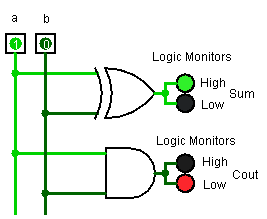
\includegraphics[width=0.5\textwidth]{part1.png}	
	\caption{Half Adder Circuit Design}
	\label{Half Adder}
\end{figure}

\paragraph{}
Truth table of the half adder that we implemented above is as below.\\\\

\begin{table}[hbt!]
\centering
    \begin{tabular}{|c|c|c|c|}
        \hline
         A & B & SUM & CARRY \\
         \hline
         0 & 0 & 0 & 0 \\
         \hline
         0 & 1 & 1 & 0 \\
         \hline
         1 & 0 & 1 & 0 \\
         \hline
         1 & 1 & 0 & 1 \\
         \hline
    \end{tabular}
    \caption{Truth table of half adder.}
    \label{table_half}
\end{table}

\clearpage
\subsection{PART 2}

\paragraph{}
In the second part of the experiment, we were expected to implement full adder. Difference between full adder and half adder is that full adder takes extra 1 input. While we can not use half adders with more than one bit operations, with that extra input, we can use full adders with n(n$\geq$1) bit operations. The full adder implementation that we did as below.\newline

\begin{figure}[!h]
	\centering
	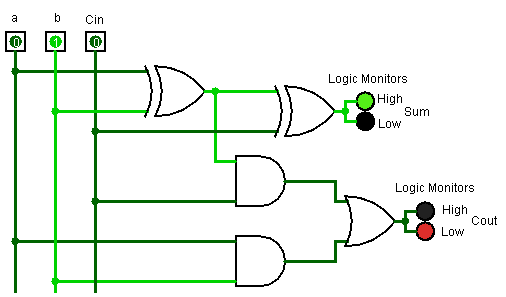
\includegraphics[width=0.7\textwidth]{part2.png}	
	\caption{Full Adder Circuit Design}
	\label{Full Adder}
\end{figure}

\paragraph{}
The truth table of the full adder is shown in Table 2 as below.\newline

\begin{table}[!h]
\begin{center}
    \begin{tabular}{|c|c|c|c|c|}
        \hline
         A & B & $C_{in}$ & $C_{out}$ & Sum \\
         \hline
         0 & 0 & 0 & 0 & 0 \\
         \hline
         0 & 0 & 1 & 0 & 1 \\
         \hline
         0 & 1 & 0 & 0 & 1 \\
         \hline
         0 & 1 & 1 & 1 & 0 \\
         \hline
         1 & 0 & 0 & 0 & 1 \\
         \hline
         1 & 0 & 1 & 1 & 0 \\
         \hline
         1 & 1 & 0 & 1 & 0 \\
         \hline   
         1 & 1 & 1 & 1 & 1 \\
         \hline         
    \end{tabular}
    \caption{Truth table of full adder.}
    \label{table_full}
\end{center}
\end{table}    
\clearpage
\subsection{PART 3}

\paragraph{}
In the third part of the experiment, we were expected to implement 4-bit full adder using full adder and XOR gates to deliver addition and subtraction operations of 4-bit signed and unsigned binary numbers. The aim of using XOR gates is to determine which operation(addition/subtraction) we are going to use. When we give 0 to $C_{in}$, our circuit will add two 4-bit binary numbers together. Since 0 $\oplus$ x = x, there will not be any complementary operation and everything is going to done properly by the circuit. When we give 1 to $C_{in}$, our circuit will subtract B from A. In order to do that, we use 2's complementary for B(2's complement of B = B' + 1). Since 1 $\oplus$ x = x', B0, B1, B2 and B3 inputs will be get complemented one by one, and $C_{in}$ value will go to the full adder as carry input again. As a result, our circuit will operate addition and subtraction operations for 4-bit signed and unsigned binary numbers successfully.

\begin{figure}[!h]
	\centering
	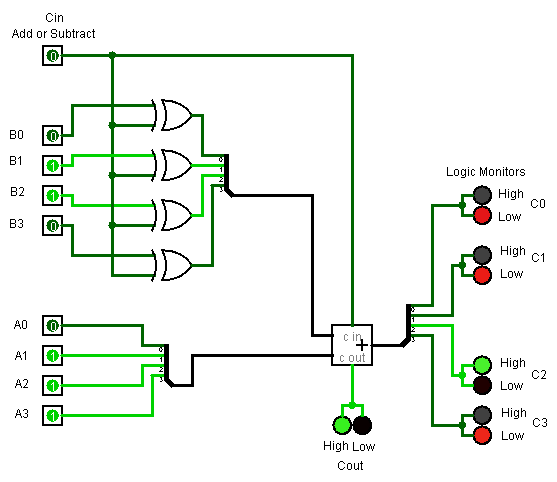
\includegraphics[width=0.7\textwidth]{part3.png}	
	\caption{4-Bit Full Adder Circuit Design}
	\label{4-Bit Full Adder}
\end{figure}
\clearpage
\paragraph{}
When we interpret A+B accepting them as unsigned binary numbers, we need to consider \textbf{carry} bit((n+1)th bit). If we get fifth bit as a result of addition, it means that we have carry bit and the result can not be represented. In other words, our numbers has to be interval of [0,15] in decimal, and any other number different from that interval can not be represented.
\paragraph{}
In Table 3, first case has not carry and it is representable. However other three cases have carry so they can not be represented. \newline
\begin{table}[!h]
\begin{center}
    \begin{tabular}{|c|c|c|c|c|}
    \hline
         A & B & Carry & Result in Binary & Result in Decimal \\
         \hline
         0101 & 0111 & 0 & 1100 & 12 \\
         \hline
         1101 & 1001 & 1 & 0110 & 22  \\
         \hline
         1111 & 1111 & 1 & 1110 & 30 \\
         \hline
         0110 & 1101 & 1 & 0011 & 19 \\
         \hline
        \end{tabular}
    \caption{Results of the unsigned sum $A + B$.}
    \label{unsigned_sum}
\end{center}
\end{table}

\paragraph{}
When we interpret A+B accepting them as signed binary numbers, we need to consider sign of the result and check if overflow exists or not. All possibilities that we need to consider for overflow situations;
\begin{itemize}
    \item positive + positive -$>$ negative
    \item negative + negative -$>$ positive 
\end{itemize}

\paragraph{}
In the Table 4, while third and fourth cases have not overflow and can be represented, first and second cases have overflow and can not be represented. \newline

\begin{table}[!h]
\begin{center}
    \begin{tabular}{|c|c|c|c|c|c|}
    \hline
         A & B & Overflow & Result sign & Result in Binary & Result in Decimal \\
         \hline
         0101 & 0111 & 1 & - & 1100 & -4 \\
         \hline
         1101 & 1001 & 1 & + & 0110 & 6 \\
         \hline
         1111 & 1111 & 0 & - & 1110 & -2 \\
         \hline
         0110 & 1101 & 0 & + & 0011 & 3 \\
         \hline
        \end{tabular}
    \caption{Results of the signed sum $A + B$.}
    \label{signed_sum}
\end{center}
\end{table}
\clearpage

When we interpret A-B accepting them as unsigned binary numbers, we need to consider borrow situation. While we subtracting two unsigned binary numbers, we have to obtain carry((n+1)th) bit. So, carry means no borrow and it is presentable while no carry means borrow and the result can not be represented.
\paragraph{}
In the Table 5, first and fourth cases have borrow, so they can not be represented while second and third cases can.\newline

\begin{table}[!h]
\begin{center}
    \begin{tabular}{|c|c|c|c|c|}
    \hline
         A & B & Borrow & Result in Binary & Result in Decimal \\
         \hline
         0101 & 0111 & 1 & 1110 & 14 \\
         \hline
         1101 & 1001 & 0 & 0100 & 4 \\
         \hline
         1111 & 1111 & 0 & 0000 & 0 \\
         \hline
         0110 & 1101 & 1 & 1001 & 9 \\
         \hline
        \end{tabular}
    \caption{Results of the unsigned subtraction $A - B$}
    \label{unsigned_subtract}
\end{center}
\end{table}

\paragraph{}
When we interpret A-B accepting them as signed binary numbers, we need to check sign of the result and check if overflow exists or not as we did it for signed A+B. All possible cases for overflow;
\begin{itemize}
    \item positive - negative -$>$ negative
    \item negative - positive -$>$ positive 
\end{itemize}

\paragraph{}In the Table 6, sign of the result of the fourth case must be positive since we subtract negative number from positive number. But we obtained negative sign, so there is overflow. Other three subtraction operation is what it has to be and there is no overflow.\newline

\begin{table}[!h]
\begin{center}
    \begin{tabular}{|c|c|c|c|c|c|}
    \hline
         A & B & Overflow & Result sign & Result in Binary & Result in Decimal \\
         \hline
         0101 & 0111 & 0 & - & 1110 & -2 \\
         \hline
         1101 & 1001 & 0 & + & 0100 & 4 \\
         \hline
         1111 & 1111 & 0 & + & 0000 & 0 \\
         \hline
         0110 & 1101 & 1 & - & 1001 & -7 \\
         \hline
        \end{tabular}
    \caption{Results of the signed subtraction $A - B$}
    \label{signed_subtraction}
\end{center}
\end{table}
\clearpage


\subsection{PART 4}
In the last part of the experiment, firstly we used Hex Inverter to use the inverse of B because of ALU outputs are in negative logic. We used 4-Bit Arithmetic Logic Unit(74xx181), a D type flipflop(74xx174), and a Hex Inverter for reaching the goal of this experiment. The ouputs are observed on the logic monitor. Input values are taken in the logic switches such as Bs and Ss. We used D type flipflop and we took the A inputs from these flipflops. Clock and M are taken from the SPDT switches. The Cn input of the ALU is taken from the power supply and is connected to ground. 

\begin{figure}[h]
    	\centering
    	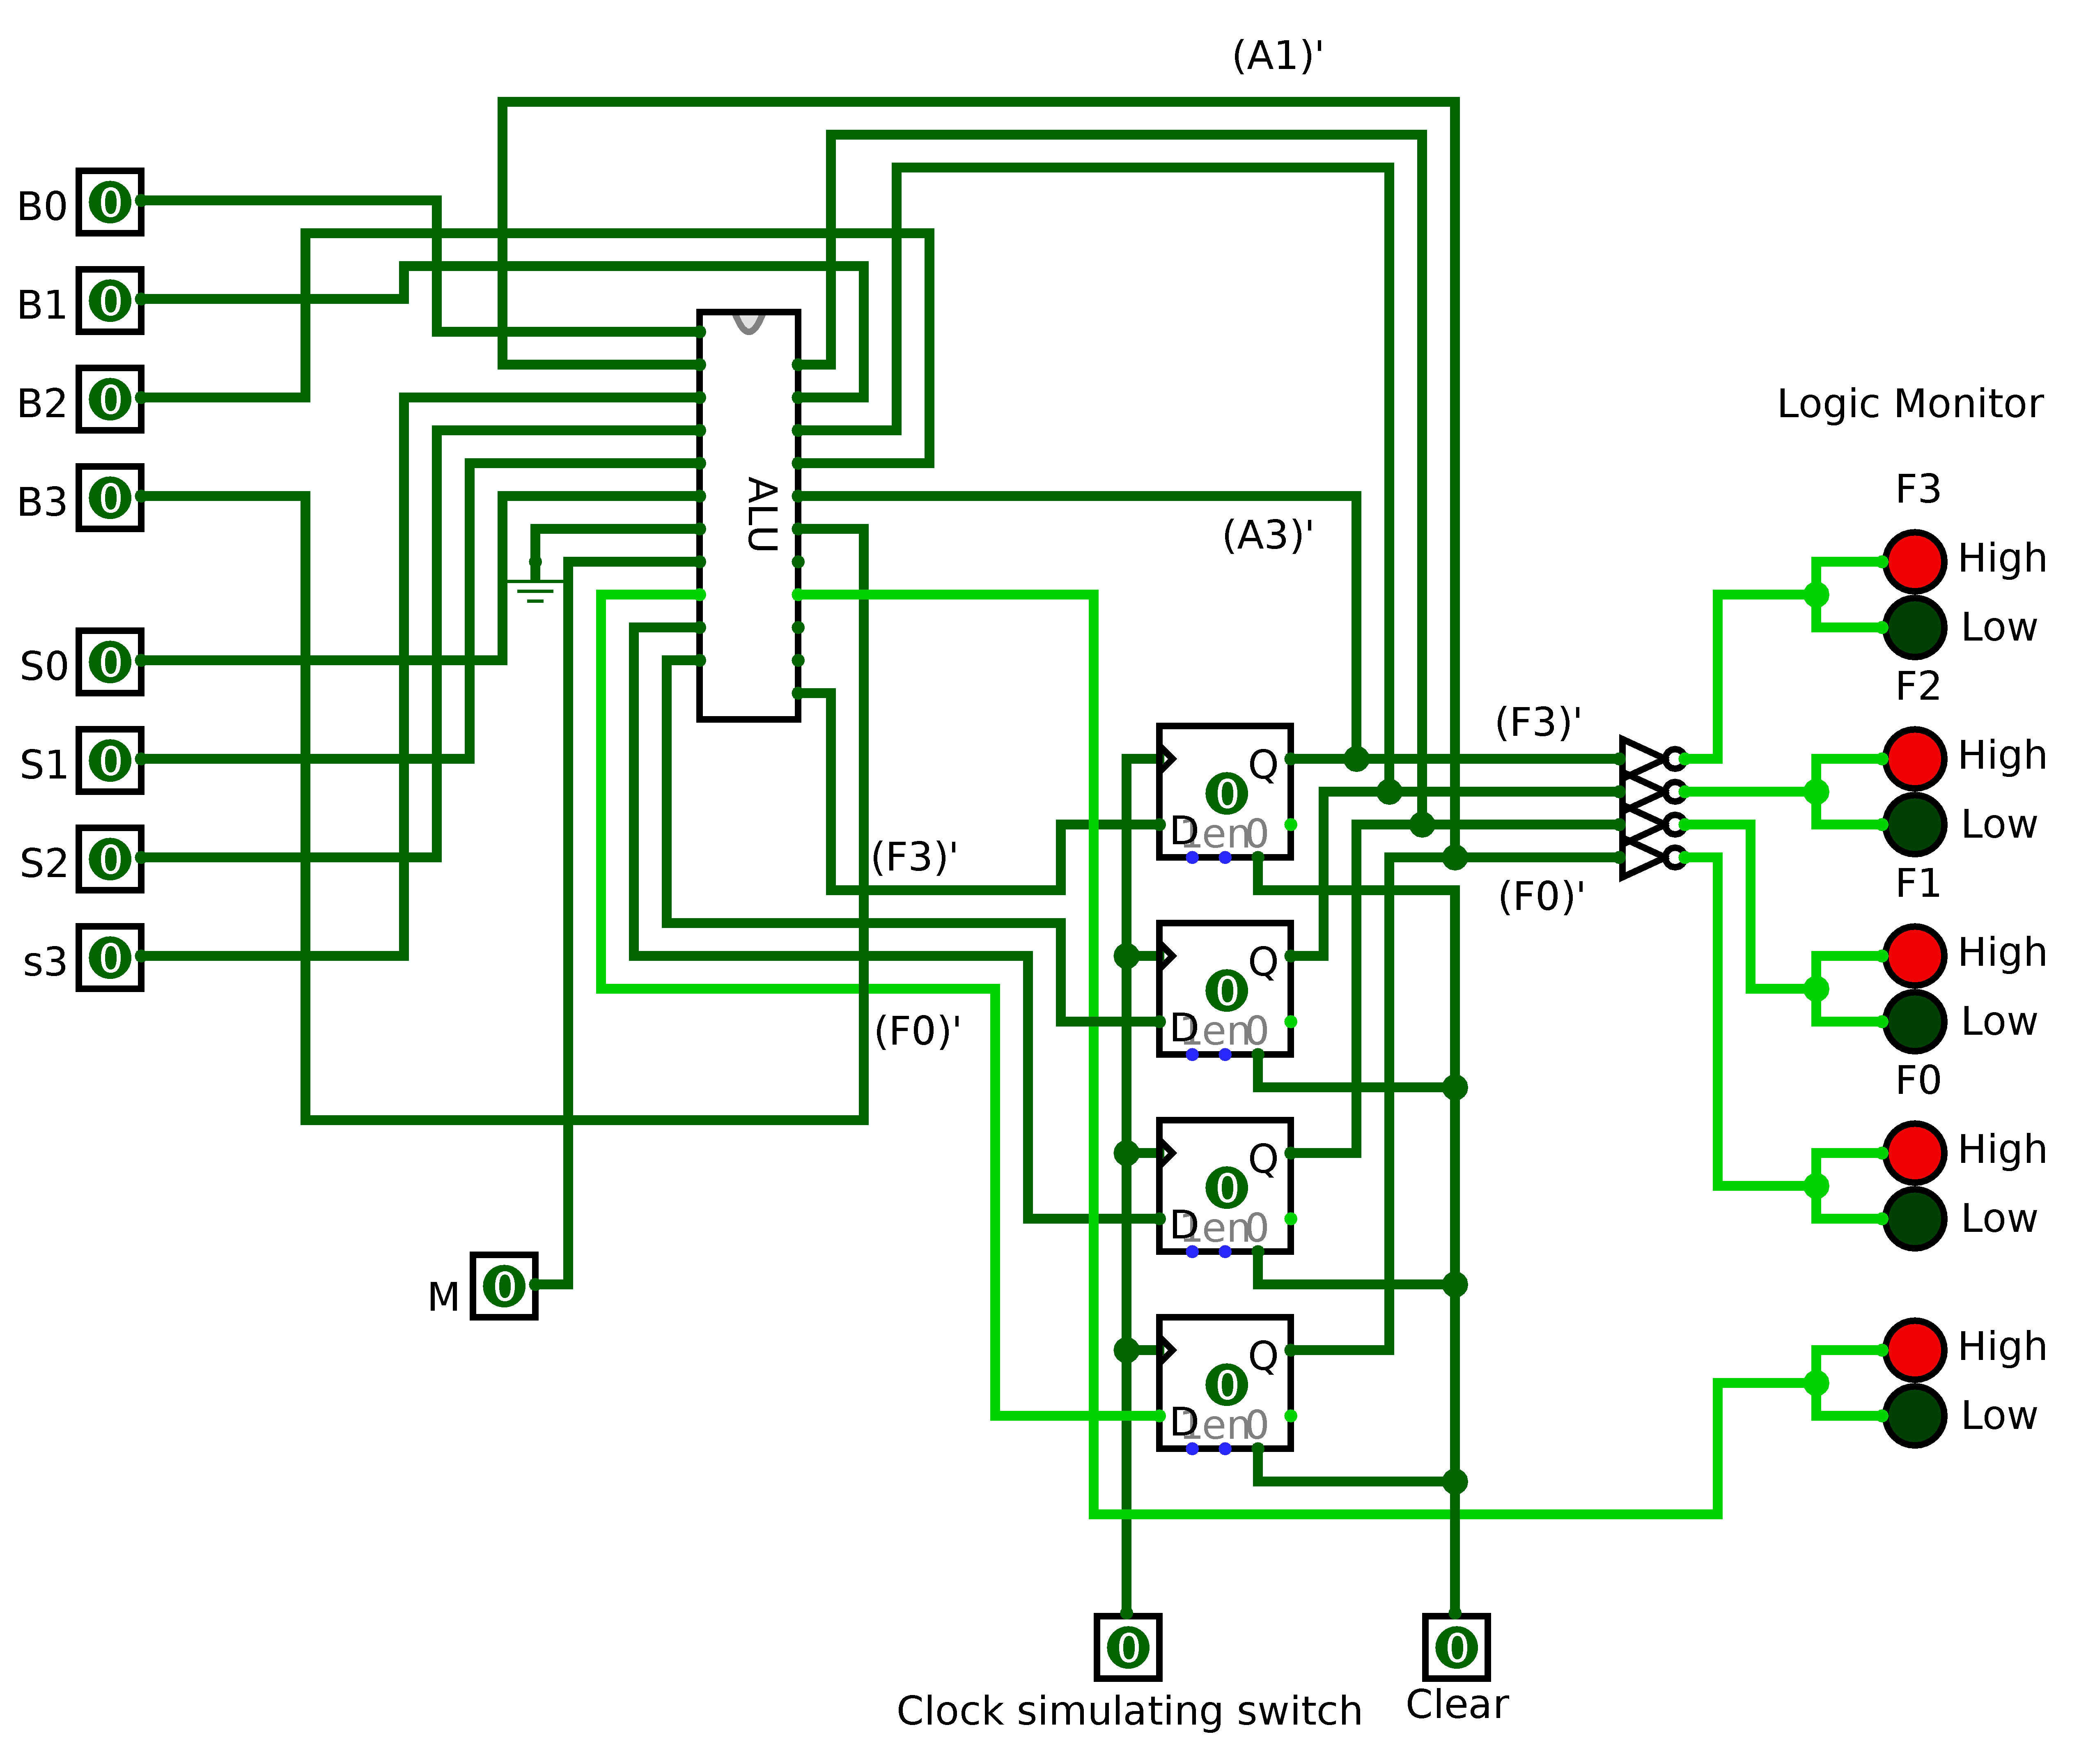
\includegraphics[width=0.8\textwidth]{part4.png}	
    	\caption{4 bit full adder (in the References)}
    	\label{fig:4-bit_full_adder}
    \end{figure}

\section{RESULTS}
Results that we obtained from the first three part of the experiment were exact same with the expected results and we verified them with the related truth tables. Therefore, there was no contradiction with the results we got. However, in the last and fourth part of the experiment, the results we obtained from our circuit design that we used ALU and D flip-flop were not matching. Results we obtained during the experiment given in the related parts in detail.
\section{DISCUSSION}
In the first part, we simply implemented half adder using an XOR and an AND gate. In the second part, we developed full adder using half adder that we did in the first part. Only difference between them is that full adder takes carry input beside two input while half adder does not. And this property allows full adder to be used in the n-bit operations while half adder can be used only for one bit operations. With this information, we implemented 4-bit full adder in the third part of the experiment. Up to now, we verified all of our output results with truth related truth tables. In the last part, we were not be able to analyze and verify our implementation because of the limited time of the session. 

\section{CONCLUSION}
As a result of the session, first three part were quite easy to handle since we had basic knowledge about the topics. As we mentioned in the results part, in the fourth part of the experiment, we implemented our design but we could not obtained expected outputs. Because of restricted time of the lab session, we could not analyze where we did something wrong and could not figure out the problem. But if we had time, we would have analyzed our implementation from starting to end carefully and could have been solve the problem. This experience taught us that we need to more and more take care of what we are going to face during the sessions.

\newpage
\addcontentsline{toc}{section}{\numberline REFERENCES}


\bibliographystyle{unsrt}
\bibliography{reference}

\nocite{booklet}
\nocite{overleaf}
\nocite{sample}


\end{document}

